\section{INTRODUCTION}
%\section*{lit review}
Coordinated conflict-free motion of a number of mobile robots in order to complete a material transfer task is important in the operation of fleets of AGV (Autonomous Guided Vehicles) used in flexible manufacturing and automated warehouses \cite{Vis2006} and \cite{Dotoli2019}. A crucial sub-problem is conflict resolution between multiple AGVs, without control of task assignment or scheduling.

It is shown, in \cite{Digani2019}, that platooning provides superior throughput to the earlier reservation based systems, and that if a solution exists it is optimal, but not that a solution exists on all roadmaps. More importantly a set of conditions which must hold for a solution to exist, is not given. The consensus algorithm in \cite{Tadano2019} also shows improved throughput in concert with a scheduling approach, but does not prove convergence. 
An example of a resolution complete algorithm based on spatial reservation is \cite{Draganjac2020}. Neither per-intersection optimal platooning nor per-vehicle consensus have been proven complete. The lack of guarantees is an important limitation of platooning methods for collision avoidance. The research gap identified is the lack of investigation into the range of motion conflict situations that can be resolved with platooning methods.

\section{Literature Review}
AGV motion coordination can be posed as a variation of the Multiple Vehicle Routing Problem with the addition of challenging spatio-temporal constraints preventing collisions between each vehicle, as well as the usual timing and capacity constraints \cite{Miyamoto2016}. In \cite{Li2017}, solutions are classified into centralized, decentralized and decoupled approaches. Each approach may be either optimal or heuristic based on whether or not they find the global minimum of some objective function. 

It is also possible to classify approaches based on the limitations they place on the state space of each AGV. Most practical methods incorporate both obstacle avoidance constraints and differential motion constraints into some sort of roadmap. This is often a graph with vertices at key points in the reachable state space, connected by edges representing feasible motion between them. The effect of increasing resolution on path quality (measured by reduction in the length of the shortest path) and computation time are studied in \cite{VanDenBerg2005}. 

Interest in centralized methods which plan in the full state space all of the vehicles was renewed by the development of effective numerical tools for operations research able to solve large combinatorial problems to optimality. Notably \cite{Richards2002} found trajectories for aircraft using a linear approximation to the dynamics and obstacle constraints, allowing the use of Mixed Integer Linear Programming. The contribution of \cite{Li2017} is to describe a new centralized, optimal method which scales well, finding a solution to the nonlinear-program for 10 vehicles in just a few seconds using an interior point method. However, size of the combined state space explodes as more vehicles are included so centralized methods are difficult to scale up to large numbers of vehicles.

Many types of decoupled methods have been developed because breaking the problem down into sub-problems is one way to reduce computation time for practical applications. Early methods of this type were based on timed petri nets \cite{Dotoli2004} and agent based models \cite{Singh2002}. Decoupled methods may sacrifice completeness (that a solution is found if one exists) in exchange for reduced average run-time. In \cite{Sanchez2002}, this was shown to cause practical difficulties in the spot-welding task studied. Spot welding requires close formation control of six vehicles, and the decoupled method frequently failed to find a solution. In \cite{Peasgood2008}, decoupled planning (incomplete) is compared with a new multi-phase heuristic, which is complete, for 50 robots on a tunnel map and 150 on an outdoor map. Decoupled planning was consistently faster in execution and produced shorter paths for lower vehicle density however it failed to find any valid paths at all for high vehicle density (25 or more robots in tunnels and 75 or more outdoors). The multi-phase heuristic, being complete, found a solution in every test case. 

More recently, \cite{Yu2013} addressed the lack of optimality in decoupled methods operating on graphs. Optimal conflict-free motion is posed as a large Integer Linear Program. Resolution complete general purpose algorithms are used to solve it for 150 robots in just over 10 seconds. The lattice/graph construction has recently been developed further to ensure kinematic constraints are met and improve coverage of state space around obstacles \cite{Yu2018}. In \cite{Miyamoto2016}, the combined problem of DCFVRP (Dispatch and Conflict-Free Vehicle Routing Problem) for flexible manufacturing is formulated as an integer program and two different decoupled algorithms are presented to solve it: local search and random search. Neither of the proposed algorithms is complete but local search found more valid solutions in the 10 random examples tested, all involving three vehicles.

Decentralized control is another option to decompose large scale problems which take too long to solve centrally \cite{Bakule2008}. Although limiting the information available to each decision maker can make reasoning about collective behavior more difficult, various attempts to decentralize conflict-free routing have been made. 
In the field of conflict free routing for mobile robots, \cite{Draganjac2016} presents a solution which generates a graph representation of the free space - effectively a roadmap - with the property of `collision-avoidability.' This means that every node on the critical path must be at most one move away from a node that does not obstruct the critical path. The critical path is defined as the union of all the shortest paths between pick/drop locations in the roadmap. During decentralized planning, AGVs attempt to reserve `private zones' consisting of the node on the critical path along with all adjacent collision avoidance nodes. Each AGV has an identical roadmap, plans the shortest path to its own goal and negotiates with those nearby based on a numeric priority to reserve the nodes in its own path. An AGV requests those in its path move to their collision avoidance node, and those with a lower priority will do so. Proof is given of correctness, that deadlocks are avoided, but throughput is sub-optimal with low priority vehicles frequently forced to stop and wait. %Another decentralized method based on sequential reservations is given by \cite{Walenta2017}, without the concept of 'private zones' to avoid deadlocks however. 
An alternative decentralized solution, based on a roadmap with two levels of detail is summarized in \cite{Sabattini2018}. Conflict-free routing primarily takes place at the most detailed level, based on prioritized roadmap reservation with local negotiation to guarantee correctness \cite{Digani2014}.  In \cite{Digani2019}, the speed of the approaching AGV is optimized at each intersection in a similar way to centralized intersection platooning. The result is higher throughput as time consuming negotiation is avoided in most cases.      

Congestion effects are represented by link performance functions in the approximate level graph. Intersections have a generalized cost which increases exponentially up to a fixed capacity which identified by parameter tuning, An optimal task scheduling approach based on the Hungarian Algorithm is used to solve the full DCFVRP in \cite{Sabattini2015a} and \cite{Sabattini2018}. Traffic delays are a type of emergent behaviour and modelling is challenging even in a completely automated system. This is the contribution of \cite{Street2020} which introduces the PRT (Probabilistic Reservation Table) to summarize the plans of robots including uncertainty so it can be in task scheduling. This approach is compared with a reservation based centralized planner as a baseline, in a simulation with 5 robots using a low level motion controller from ROS (Robot Operating System) which often fails at when two robots plan interfering paths. Congestion aware planning leads to fewer failures of the low level controller than independent planning but more than centralized planning. A more convincing comparison would be with a congestion aware planner using a deterministic congestion model instead of the PRT, but this is not reported.

Intersection control, based on platooning, is a concept developed for the operation of anticipated CARVs (Connected and Autonomous Road Vehicles). A recent review of approaches for intersection and merging coordination is given in \cite{Rios-Torres2017}. Centralized optimization approaches improve on early ideas like First-Come-First-Served spatial reservation from \cite{Dresner2008} by minimizing fuel consumption, but the rapid increase in state space with larger numbers of vehicles will need to be addressed before large scale adoption. The communication channel connecting every vehicle with the central controller introduces a single point of failure, the reliability effect of which is difficult to evaluate in existing simulations. Moreover there are few CARVs available making a practical experiment unfeasible in most cases. Attempting to address these limitations are decentralized methods such as fuzzy-logic, virtual vehicle platooning and invariant set approaches. Notably the conditions for solutions to exist which minimize energy consumption are given in \cite{Malikopoulos2018}.

Recently \cite{Tadano2019} described an approach to the DCFVRP for flexible manufacturing based on dynamic platooning with vehicle-to-everything messaging and consensus speed control, resulting in a decentralized heuristic solution with some additional rules to ensure correct behavior and avoid deadlocks by adding a reservation protocol for some parts of the roadmap. This was combined with feedback from the queue length at different workstations in a traffic management heuristic. Simulation results show an impressive improvement compared to the first-come-first-served scheduling approach meant to represent industry standard practice.   

A promising approach for intersection control applied to AGV is given in \cite{Digani2019}. As the paths are not modified, only the speed adjusted deadlocks are proved impossible. However, a backup system based on negotiation is still required because the problem is non-convex suggesting a feasible solution may not be found in time for certain roadmap and traffic combinations. The consensus based platooning method for local collision avoidance used in \cite{Tadano2019} is unusual in the AGV domain. That work makes no claims about completeness, but does consider the trivial consensus where all vehicles stop in a deadlock. In \cite{Zhang2018}, a recent system for conflict avoidance based on time headway is shown to significantly reduce intersection crossing time and allow more vehicles to operate in the same floor-space compared to a traditional reservation based strategy. Of these different approaches to platooning for AGV coordination, the quadratic constraints of \cite{Digani2019} are the closest to acheiving the certainty the would be required to build a distributed coordination scheme.
%\section{METHODOLOGY}
%
%With existing methods, a backup system is needed to prevent collisions in exceptional cases, as there is no proof of completeness of the main algorithm. A proof might be possible placing certain conditions on the traffic flow or the roadmap layout, but this is left for further work. Instead we focus on simulation to identify situations where convergence is more or less reliable. This will help to identify sites where the potrential throughput benefiits can be realized because the slower fallback option will be needed less often. It may also highlight situations in which current methods frequently fail, and help to inform modified algorithms to address these cases.  

%\begin{figure}[htbp]
%\centerline{\includegraphics[width=1.0\linewidth]{single-track-layout.png}}
%\caption{Single-track grid layout}
%\label{fig:single-track-layout}
%\end{figure}
%%[htbp]
%%\scalebox{0.5}[heightscale]{}
%%\resizebox{1.0\linewidth}{1.0\linewidth} %only for \include{graphics}
%%\centerline{\includegraphics[width=1.0\linewidth]{single-track-layout.png}}
%\begin{figure}[htbp]
%\centerline{\includegraphics[width=1.0\linewidth]{highway-layout.png}}
%\caption{Highway grid layout.}
%\label{fig:highway-layout}
%\end{figure}

%To test the success rate in finding a solution from a variety of initial conditions, we assume all AMR follow their planned trajectory exactly and look for cases where the platooning algorithm did not converge before the intersection, leading to a collision. The trajectory of each AMR must be tracked over time at a relatively high frequency, such as 10hz. Circular bodies of fixed radius can be assumed to make collision checking straightforward. Lateral dynamics can be neglected by assuming the path following controller is successful and tracks the path exactly.  Second order dynamics enable comparison of energy consumption resulting from platooning. Deadlocks and Live-locks can both be checked based on a time threshold for a vehicle to complete a job e.g. the transfer time plus the length of time it would take a vehicle to traverse the entire roadmap. If either is exceeded the simulation state should be recorded for further analysis. 
%
%In order to do this a number of realistic roadmaps are required, along with sensible parameters for vehicle size, acceleration and top speed. These can be estimated based on the literature such as \cite{Boysen2019} and \cite{Dotoli2019}. Important classes of roadmap which may be representative include grids, one-way aisles and two-way aisles.  such as those in Figures \ref{fig:single-track-layout} and \ref{fig:highway-layout}. 


%Conflict avoidance is only one part of the DVFVRP problem, the job assignment method has a profound affect on the frequency and complexity of the motion conflicts which need to be resolved. For this reason it is important to track genuine transfer jobs, assigned to a fixed number of `physical' vehicles (they do not appear and disappear at convenient times and move only according to a second order dynamic model). There is a separate question of which job scheduling algorithm and associated traffic model is best suited to each conflict-resolution method which we will not address here. For simplicity of exposition and ease of reproduction we will use a nearest-first-come-first-served scheduling approach to create traffic for both conflict-resolution methods. This is sufficient that the  number of transfer tasks completed can be tracked in a simulation of `physical' vehicles. Improvement of productivity using a traffic model and the Hungarian algorithm (e.g. \cite{Sabattini2015a}) is left for further work. We know of no reason it would benefit one method in particular.

\section{Method}
Platooning with speed choice by a centralized controller was implemented with a vehicle to intersection messaging scheme. The full site is divided into zones, each one containing a single intersection. Each AGV in the fleet has a copy of the roadmap which is  static. The fleet controller interfaces with the warehouse management system to get the next material transfer job, consisting of a pick location and a drop location. All jobs are assumed to be of unit size and each AGV has a capacity of one unit. With these assumptions, a straightforward policy is to assign the next job to the AGV nearest to the pick location - first-come-first-served scheduling. When an AGV receives a new job, it finds the shortest path through the roadmap using the Floyd-Warshall algorithm \cite{Djojo2013}. Next it must send its planned path to the intersection controller for the zone it currently occupies. The intersection controller stores the plan and current position of every AGV approaching the conflict point of the intersection. Every time it receives a new plan it must recalculate the approach speed for every approaching AGV to minimize total travel time without collision. This will happen every time an AGV enters the zone from somewhere else, or an AGV within the zone is assigned a new job.

%\begin{figure}[ht]
%\centering
%\includegraphics[width=\linewidth]{intersection_layout_trim}
%\caption{Intersection layout shown in SUMO NETEDIT tool \cite{dlr2016}}
%\label{fig:layout}
%\end{figure}
\begin{figure}[ht]
\centering
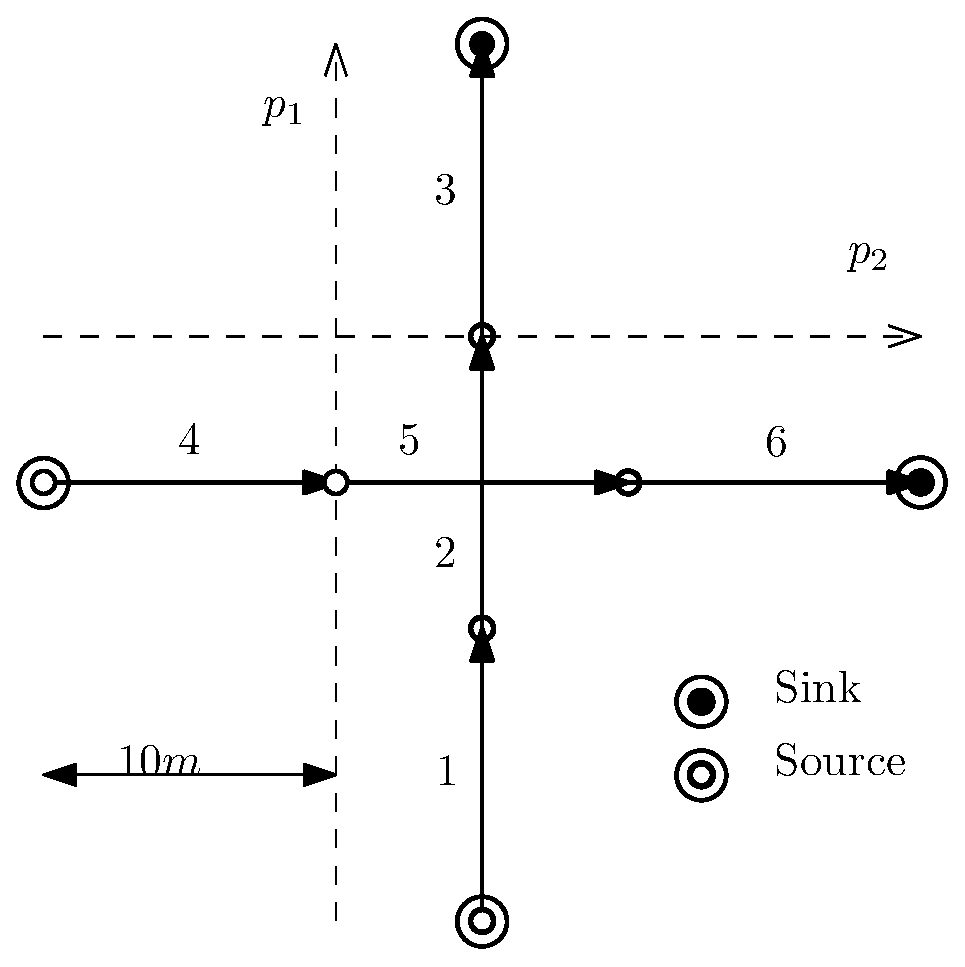
\includegraphics[width=\linewidth]{intersection_topo}
\caption{Intersection layout with two conflicting routes.}
\label{fig:layout}
\end{figure}

The intersection controller was implemented based on \cite{Digani2019}. The surrounding lanes are first discretized into segments. The intersection shown in Figure \ref{fig:layout} is divided into six segments, each of length 10 meters. The critical segments are the two that cross in the center. There are two routes defined, one starting on the left and traveling to the right and the other starting at the bottom and traveling up. One AGV takes route 1 and the other takes route 2. If they both travel at maximum speed they will collide in the center.

The dynamic model for each AGV assumes they are able to exactly follow the path, and attempt to reach the target speed for each segment subject to a limited rate of acceleration of $a m/s^2$. 

\begin{figure}[ht]
\centering
\includegraphics[width=\linewidth]{SystemSetup3.pdf}
\caption{Messages exchanged by participants approaching intersection.}
\label{fig:system_setup}
\end{figure}

The ApproachPlan message sent by the AGV contains a sequence of segments which it intends to traverse, along with its current distance along the first one.  The flow of messages is shown in Figure \ref{fig:system_setup}. The SpeedList sent by the intersection controller contains the optimal speed for every segment in the plan. The speeds can be found with the nonlinear program in Equation \ref{eq:qp_speeds}. 

\subsection{Intersection Controller Objective}
The objective is to minimize $J_T$ the total travel time for all vehicles. It is convenient for exposition to optimize over the inverse of speed of each segment $\phi_k = 1/v_k$. Vehicle $i$ submits a plan containing $m_i$ segments before the conflict and $n_i$ segments in conflict. The control model is based on the average speed of each approaching AGV over each segment. This is to simplify the description of the intersection controller, and assist analysis. More sophisticated motion models could take the place of  Equation \ref{eq:omega_min} and  Equation \ref{eq:omega_max} to create a similar type of problem with a convex travel time objective and non-convex constraints.   
The parameters for one vehicle can be collected in the vector $\bm{\phi}_i$ as shown in Equation \ref{eq:phi_i}
\begin{equation}
\bm{\phi}_i =  [\phi_{1}, ..., \phi_{(m_i + n_i)}]^T \\
\label{eq:phi_i}
\end{equation}
The parameters for $p$ vehicles each traversing $(m_i + n_i)$ segments are assembled into a vector as in Equation \ref{eq:parameters}
\begin{equation}
\bm{\phi} = [\bm{\phi_{1}}^T, ..., \bm{\phi}_{p}^T]^T \\
\label{eq:parameters}
\end{equation}
Similarly, the length of each segment in plan $i$ can be arranged into a vector 
\begin{equation}
\bm{d}_i = [d_{1}, ..., d_{(m_i + n_i)}]^T \\
\label{eq:d_i}
\end{equation}
and collected  for $p$ vehicles into a vector as in Equation \ref{eq:d}.
\begin{equation}
\bm{d} = [\bm{d_{1}}^T, ..., \bm{d}_{p}^T]^T \\
\label{eq:d}
\end{equation}
This leads to the minimum travel time objective in Equation \ref{eq:qp_speeds}. 
\begin{equation}
\begin{array}{c}
\min \limits_{\bm{\phi}} \bm{J_T} = \bm{d}^T \bm{\phi} \\
\textrm{subject to}\\
 \bm{\phi}_{max} > \bm{\phi} > \bm{\phi}_{min} \\
 \bm{\phi}^T\bm{H}_{i,j}\bm{\phi} > \bm{0} \quad \forall i,j \in [1,p] \quad \textrm{with } j>i \\
\end{array}
\label{eq:qp_speeds}
\end{equation}

The condition $j>i$ in Equation \ref{eq:qp_speeds} indicates that the number of constraints varies with the number of vehicles $p$ as $\frac{p(p-1)}{2}$. This corresponds to one constraint between each pair of approaching AGVs.

\subsection{Intersection Controller Timing Constraints}
By definition, each intersection has a single conflict zone, the union of all segments which intersect there. This makes it possible to express the constraint that vehicles do not collide in terms of time. Vehicle $i$ arrives at the first conflicted segment $\omega_i^{min}$ and departs from the last at $\omega_i^{max}$. The following three subsections set out three alternative ways of expressing the collision avoidance constraints which have been evaluated. 
The arrival time is given by Equation \ref{eq:omega_min}. Considering average speeds, the departure time $\omega_i^{max}$ is also linear, this is given by Equation \ref{eq:omega_max}. 
\begin{equation}
\omega_i^{min}  = \sum_{k=1}^{m_i} \bm{d}_i [k] \bm{\phi}_i [k] = \bm{e}^T \bm{\phi}_i
\label{eq:omega_min}
\end{equation}
where %$\bm{e}[k] = \bm{d}_i[k] \forall k <m_i, otherwise 0$
\begin{equation}
\bm{e}[k] = \left\{
\begin{array}{cc}
\bm{d_i}[k] & \forall k <m_i \\
0 & \textrm{otherwise} \\
\end{array}
\right.
\end{equation}  and $m_i$ is the number of segments on the path of vehicle $i$ before arrival at the conflicted segment. 
\begin{equation}
\omega_i^{max}  = \omega_i^{min} + \sum_{i=1}^{n_i} \bm{d}_i [k] \bm{\phi}_i [k] = \bm{f}^T \bm{\phi}_i
\label{eq:omega_max}
\end{equation}
where 
\begin{equation}
\bm{f}[k] = \left\{
\begin{array}{cc}
\bm{d_i}[k] & \forall k <m_i+n_i \\
0 & \textrm{otherwise} 
\end{array}
\right.
\end{equation}
 and $n_i$ is the number of segments on the path of vehicle $i$ which are conflicted. Note that Equations \ref{eq:omega_min} and \ref{eq:omega_max} only depend on the $\bm{\phi}_i$ of vehicle $i$. 



\subsubsection{Linear FIFO Constraints}
\label{sec:fifo_constraints}
If the order in which the AGV cross the conflict zone is fixed to be First-In-First-Out, the timing constraint is linear. There is one constraint between each adjacent pair so $p-1$ constraints total for $p$ vehicles. These can be expressed in the form $\bm{A}_{ub}\phi \leq \bm{b}_{ub}$  as in Equation \ref{eq:fifo}. This is correct for two AGV arranged in distance order, each traversing one approach and one conflict segment. 

\begin{equation}
\left[ 
\begin{array}{ccccc}
-d_1 & 0 & d_3 & d_4 \\
\vdots 
\end{array} \right]
\left[
 \begin{array}{c}
  \phi_1 \\ \phi_2 \\ \phi_3 \\ \phi_4
 \end{array} \right]
\leq
\left[ 
\begin{array}{c}
0 \\ \vdots
\end{array} \right]
\label{eq:fifo}
\end{equation}

 The timing constriant between each pair of vehicles can be expressed with a modulus operator as in Equation\ref{eq:timing}.
\begin{equation}
|\alpha_i - \alpha_j| > \beta_i + \beta_j
\label{eq:timing}
\end{equation}

Here 
\begin{equation}
\alpha_i  = \omega_i^{max} + \omega_i^{min}
\label{eq:alpha}
\end{equation}
represents the midpoint of the time vehicle $i$ occupies the conflicted segment and
\begin{equation}
\beta_i  = \omega_i^{max} - \omega_i^{min}
\label{eq:beta}
\end{equation}
represents the range of the time either side of the midpoint, both scaled by a factor of two. 


In matrix form
\begin{equation}
\alpha_i  = \bm{f}^T \bm{\phi}_i + \bm{e}^T \bm{\phi}_i = \bm{1}_i^T\bm{A}{\phi}_i
\label{eq:alpha_m}
\end{equation}
with $\bm{A} = diag(\bm{f} + \bm{e})$
\begin{equation}
\beta_i  = \bm{f}^T \bm{\phi}_i - \bm{e}^T \bm{\phi}_i =  \bm{1}_i^T\bm{B}{\phi}_i
\label{eq:beta_m}
\end{equation}
with $\bm{B} = diag(\bm{f} - \bm{e})$

The resulting linear program (with parameters $\in\mathbb{R}$) has $p-1$ constraints as each AGV is only constrained by the preceeding one.

\subsubsection{Quadratic Constraints}
\label{sec:quad_constraints}
Another way to treat the modulus operator in Equation \ref{eq:timing}, without forcing any particular arrival order is to square both sides as to give the expression in Equation \ref{eq:expanded}. 
\begin{equation}
\alpha_i^2 - \alpha_j^2 - 2 \alpha_i\alpha_j - (\beta_i^2 + \beta_j^2 +2 \beta_i \beta_j) > 0
\label{eq:expanded}
\end{equation}
Collecting terms by subscript gives
\begin{equation}
(\alpha_i^2 - \beta_i^2) - (\alpha_j^2 + \beta_j^2) - 2(\alpha_i\alpha_j + \beta_i \beta_j) > 0
\label{eq:collected}
\end{equation}

The matrix $\bm{\Lambda}_ij$ captures the constraints between a pair of vehicles and always contains four sub-matrices as shown in in Equation \ref{eq:lambda}. It is compatible with $\bm{\phi}_{i,j} = [\bm{\phi}_i^T, \bm{\phi}_j^T]^T$, containing only the relevant speeds for vehicles $i$ and $j$. 
\begin{equation}
\bm{\Lambda}_{ij} =\left[
	\begin{array}{cc}
\bm{\Lambda}_{ij}^{ii} & \bm{\Lambda}_{ij}^{ij} \\
\bm{\Lambda}_{ij}^{ji} & \bm{\Lambda}_{ij}^{jj} \\
	\end{array}
	\right]
\label{eq:lambda}
\end{equation}
Expanding 
\begin{multline}
\left[\bm{\phi}_i^T, \bm{\phi}_j^T\right]
 \left[\begin{array}{cc}
\bm{\Lambda}_{ij}^{ii} & \bm{\Lambda}_{ij}^{ij} \\
\bm{\Lambda}_{ij}^{ji} & \bm{\Lambda}_{ij}^{jj} \\
	\end{array}\right]
\left[\begin{array}{c}
\bm{\phi}_i\\
 \bm{\phi}_j \end{array} \right] \\
= \bm{\phi}_{i}^T \bm{\Lambda}_{ij}^{ii} \bm{\phi}_{i} + \bm{\phi}_{j}^T \bm{\Lambda}_{ij}^{jj} \bm{\phi}_{j} + \bm{\phi}_{i}^T \bm{\Lambda}_{ij}^{ij} \bm{\phi}_{j} + \bm{\phi}_{j}^T \bm{\Lambda}_{ij}^{ji} \bm{\phi}_{i}
\end{multline}
 makes it possible to compare terms with the scalar expression in Equation \ref{eq:collected}. This leads to the following expressions for the submatrices in $\Lambda$ in terms of $\alpha_i = \bm{1}_T\bm{A}_i\bm{\phi}_i$ and $\beta_i = \bm{1}_T\bm{B}_i\bm{\phi}_i$ 
\begin{equation}
\bm{\Lambda}_{ij}^{ii} = (\bm{A}_i - \bm{B}_i)\bm{1}_i\bm{1}_i^T(\bm{A}_i - \bm{B}_i) 
\label{eq:ii}
\end{equation}
\begin{equation}
\bm{\Lambda}_{ij}^{jj} = -(\bm{A}_j + \bm{B}_j)\bm{1}_j\bm{1}_j^T(\bm{A}_J + \bm{B}_j) 
\label{eq:jj}
\end{equation}
\begin{equation}
\bm{\Lambda}_{ij}^{ij} + \bm{\Lambda}_{ij}^{ij T} = -2(\bm{A}_j + \bm{B}_j)\bm{1}_j\bm{1}_i^T(\bm{A}_i + \bm{B}_i) 
\label{eq:ij}
\end{equation}

For more than two vehicles this can be arranged into a block diagonal matrix $\bm{H}_{ij}$ which is compatible with the input parameters, but still only represents the constraints between a pair. 

Expressed in this way it is clear the constraints are quadratic and it is trivial to differentiate twice to find the Hessian is the stack of constraint matrices $[\bm{H}_{ij}, \hdots]$. The objective is certainly convex as it is linear but the constraints may not be. If the Hessian of the constraints is positive semi-definite then they are convex and interior point methods will either find the global optimum or prove that there is no feasible solution \cite{Boyd2004}. The Hessian depends on the parameters of the roadmap, the number of approaching vehicles and their distance from the conflict. 

\subsubsection{Mixed Integer Constraints}
\label{sec:milp_constraints}
A third way of treating the timing constraint in Equation \ref{eq:timing}, also without forcing any particular arrival order involves splitting each constraint into two based on the sign of $(\alpha_i-\alpha_j)$ as shown in equation \ref{eq:or_cons}. Again, this is expressed in terms of the midpoint $\alpha_i$, $\alpha_j$ and extent $\beta_i$,$\beta_j$ of the time when vehicle $i$ and vehicle $j$ occupy the segment on their own path which passes through the conflict point,
\begin{equation}
\begin{array}{cc}
\alpha_i - \alpha_j > \beta_i + \beta_j &\textrm{if  }\alpha_i >\alpha_j  \\
\alpha_i - \alpha_j < -(\beta_i + \beta_j) & \textrm{otherwise}\\
\textrm{where } \alpha_i, \alpha_j, \beta_i, \beta_j >0
\end{array}
\label{eq:or_cons}
\end{equation}
In order to apply these OR constraints, an additional integer parameter $b_k$ can be introduced for each pair of AGV, along with an arbitrary large number $M$ as shown in Equation \ref{eq:big_m_cons}. 
\begin{equation}
\begin{array}{cc}
\alpha_i - \alpha_j + b_{i,j}M > \beta_i + \beta_j \\
\alpha_i - \alpha_j - (1-b_{i,j})M < -(\beta_i + \beta_j) \\
\textrm{where } b_{i,j}\in[0,1] \\
M>>\alpha_i, \alpha_j, \beta_i, \beta_j
\end{array}
\label{eq:big_m_cons}
\end{equation}
Now the problem is combinatorial rather than convex and appropriate methods must be used. These may be based on exhaustive search such as Branch-and-Bound, or solving a sequence of convex relaxations of the original problem \cite{Murray2010}. Combinatorial problems quickly become intractable for large numbers of variables, but in this case the underlying problem of arrival order is combinatorial, so exhaustive methods are needed to find the global minimum. 

It is possible to further assume every AGV travels at maximum speed once it reaches the conflict, simplifying equation Equations \ref{eq:alpha} and \ref{eq:beta} with a constant $p_i = g_i \phi_{min}$. 
\begin{equation}
\alpha_i = 2\omega_i^{min} + p_i
\end{equation}
\begin{equation}
\beta_i = p_i
\end{equation}
 where $g_i$ is the length of the conflicted segments in the plan of vehicle $i$. In this case Equation \ref{eq:big_m_cons} can be restated 
\begin{equation}
\begin{array}{cc}
\omega_i^{min} - \omega_j^{min} + b_{i,j}M > p_j \\
\omega_i^{min} - \omega_j^{min}  - (1-b_{i,j})M < -p_i \\
\textrm{where } b_{i,j}\in[0,1] \\
\end{array}
\label{eq:minlp}
\end{equation}